% ----------------------------------------------------------
% Introdução 
% Capítulo sem numeração, mas presente no Sumário
% ----------------------------------------------------------

\chapter[Introdução]{Introdução}

Nos últimos anos, os termos, aprendizado de máquina e aprendizado profundo, ficaram populares e já estão presentes em soluções 
disponíveis para o público geral, desde a assistente virtual dos dispositivos móveis e eletrônicos de consumo, até sistemas capazes 
de embasar diagnósticos médicos, como, por exemplo, uma aplicação capaz de auxiliar em diagnósticos de COVID-19 durante a pandemia do 
vírus SARS-COV2 [\citeonline{Zhao2021DeepLF}]. São conceitos utilizados em aplicações de diversos segmentos, sendo um especialmente 
importante para esse trabalho de graduação, o de processamento de imagem. Alguns exemplos de funcionalidades atuais 
que, de alguma forma, se apoiaram em conceitos e técnicas relacionados ao aprendizado de máquina são funcionalidades “modo retrato” [\citeonline{GooglePortrait}] 
e “modo noturno” [\citeonline{GoogleLowLight}] do aplicativo de câmera de dispositivos móveis, sendo que as referências citadas documentam 
os estudos dessas funcionalidades em dispositivos da linha Pixel, desenhados pela Google.

Um escopo em particular de aplicação de técnicas de aprendizado de máquina que evoluiu com o crescimento da popularidade e 
acessibilidade dos conceitos que envolvem aprendizado de máquina são aplicações voltadas para reconhecimento de texto. 

A escrita com certeza foi uma das grandes habilidades que a humanidade desenvolveu que mudou como relações e sociedades funcionavam, adotada 
para transmissão e armazenagem de dados e informação, meio de comunicação e expressão.

Com os avanços da tecnologia e em especial, dos computadores, um grande desafio emergiu: como fazer com que computadores entendam o que está 
escrito em documentos físicos? Umas das primeiras patentes para soluções de OCR (abreviação de \textit{Optical Character Recognition}) data 
de 1929 [\citeonline{readingMachine}], mas isso não nega o fato que a capacidade de transportar texto do meio físico para o meio digital de 
forma eficiente é um desafio interessante e motiva pesquisas até hoje.

Em linhas gerais, o reconhecimento óptico de caracteres é uma ampla tarefa de reconhecimento de padrões e, para que máquinas consigam identificar 
os padrões presentes nas instâncias de texto, elas precisam conhecer ao menos algumas características dos caracteres e do texto que serão 
reconhecidos. Para exemplificar, a \textit{Reading Machine} [\citeonline{readingMachine}], proposta por Gustav Tauschek, era um aparelho mecânico que utilizava um disco de 
comparação, que guardava o gabarito de cada um dos caracteres do alfabeto suportado. Esse foi o meio de “ensinar” a máquina a reconhecer um dado carácter.

Muitos anos depois, soluções ainda tem a missão de “treinar” computadores a identificar as características de caracteres e de textos na totalidade 
e a principal ferramenta utilizada atualmente são métodos sob o domínio do aprendizado de máquina, justamente pela capacidade de predição desses 
algoritmos dado um processo de treinamento. Ao longo deste trabalho de graduação outros conceitos que circundam o tópico de aprendizado de máquina 
serão introduzidos com um pouco mais de profundidade.

\section{\textit{Scene Text Recognition}}

Um sub-conjunto de casos do espaço de aplicações de reconhecimento óptico de caracteres ganhou tração na última década, impulsionada pelo 
alto poder computacional dos dispositivos modernos, acelerados por unidades gráficas, e a acessibilidade ao desenvolvimento de soluções de aprendizado 
de máquina. Esse sub-conjunto é conhecido como STR, abreviação no nome em inglês \textit{Scene Text Recognition}. Uma analogia para o STR seria aplicar 
soluções de OCR diretamente de fotos capturadas por uma câmera de um dispositivo móvel. Algumas soluções acessíveis ao público geral que lidam 
com STR pode-se citar aplicações como o \textit{Google Lens} e o \textit{Apple Live Text}, que permitem a extração de texto de imagens diretamente 
da câmera do dispositivo móvel, muitas vezes em situações similares aos que são explorados nos trabalhos que procuram resolver o reconhecimento 
de texto em cenas.
 
A principal diferença entre um problema de STR comparado ao caso mais comum de OCR é, em termos simples, a aparência do texto e como ele será observado. 
Em uma imagem de cena, como, por exemplo, uma imagem da faixada de um supermercado ou comércio, ilustrado pela Figura \ref{fig:str-example}, podemos 
ter textos em diferentes tamanhos, com diversas fontes, cores e orientações. Adicionalmente, por estarem muitas vezes sob influência do ambiente onde 
estão inseridos, outros fatores influenciam a observação desse texto, como iluminação, oclusão, danos devido ao clima, etc.

\begin{figure}
    \centering
    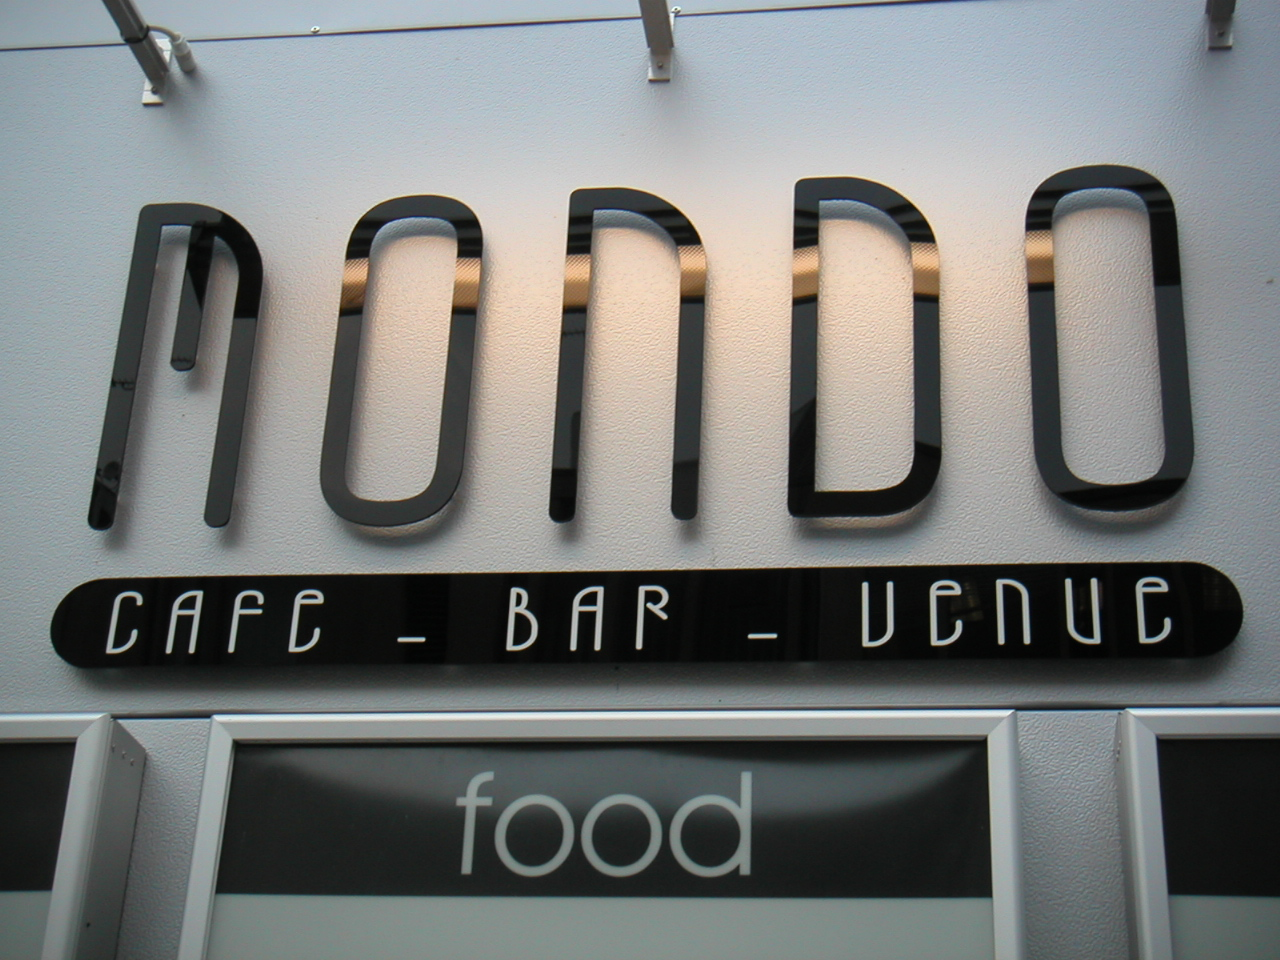
\includegraphics[width=0.75\textwidth]{figs/img_139.jpg}
    \caption{Imagem de uma faixada de comércio, ilustrando um caso de STR. Fonte [\citeonline{ICDAR2013}]}
    \label{fig:str-example}
\end{figure}

As soluções para problemas de STR, para lidarem com o nível de generalização necessário para reconhecer texto nos mais diversos casos, são largamente 
baseadas nos conceitos de aprendizado profundo, que demonstram conseguir ir um passo à frente no quesito reconhecimento de padrões em comparação às 
técnicas clássicas de processamento de imagem. O uso em especial das redes neurais convolucionais, 
comumente abreviadas para CNN pelo nome em inglês \textit{Convolutional Neural Networks}, um divisor de águas na evolução dessas soluções. 
[\citeonline{DetcRecogWild,StrDlEra}]. A própria aplicação \textit{Google Lens}, citada anteriormente, utiliza redes convolucionais baseadas em RPN (\textit{Region Proposal Networks)} e redes recorrentes do tipo LSTM (\textit{Long Short-Term Memory}) para detectar e reconhecer texto nas imagens enviadas pelos usuários [\citeonline{GoogleLens}].

A popular biblioteca OpenCV\footnote{https://opencv.org/} é uma porta de entrada para iniciantes experimentares soluções de detecção e reconhecimento de texto mais robustas. No módulo de redes neurais profundas da biblioteca, é disponibilizado ferramentas para executar modelos pré-treinados de detecção e de reconhecimento de texto, compatíveis com trabalhos relevantes na área, como EAST [\citeonline{EAST}] e o CRNN [\citeonline{CRNN}], por exemplo.

A pesquisa e experimentação de novos métodos para resolver os mais diferentes problemas que permeiam o STR ainda é atual, com trabalhos 
publicados recentemente.
Em [\citeonline{KPN}], por exemplo, é proposta uma nova arquitetura de detecção, abreviada por KPN pelo nome em inglês \textit{Kernel Proposal Network}), 
utilizando redes convolucionais e segmentação semântica para melhorar a detecção das fronteiras de palavras.

Já em [\citeonline{DEER}], uma solução unificada de localização e reconhecimento é sugerida utilizando redes convolucionais inspirada em soluções de 
detecção de objetos baseadas em codificadores \textit{Transformers} [\citeonline{Transformer}], que, no que lhes concerne, utilizam métodos de atenção. 
As regiões de texto são localizadas apenas por um ponto de referência central, não por uma área bem definidas como é comum. Posteriormente um decodificador 
é utilizado para gerar a sequência de caracteres no entrono do ponto de referência.

\section{Objetivo}

O principal objetivo deste trabalho de graduação é desenvolver e avaliar uma solução integrada de reconhecimento de texto em cenas a parir do uso de 
componentes para detecção e reconhecimento isolados que já fizeram parte do estado da arte, respectivamente CRAFT e CRNN.

Como objetivo complementar, de modo a gerar uma prova de conceito sobre a solução desenvolvida, a partir do uso de provedores de computação em nuvem, 
hospedar uma aplicação \textit{web} para disponibilizar o uso da solução desenvolvida na Internet.

\section{Considerações finais}
Dada a importância do aprendizado profundo, e em especial das CNNs nesse contexto de detecção e reconhecimento de texto, o próximo capítulo irá 
apresentar alguns conceitos básicos associados a essas estruturas.